\section{实验}
\label{sec:experiments}

如第~\ref{sec:indomain_ood_sft} 节所示，PivotRL 相比同数据 SFT 带来了更大的域内收益，同时几乎消除了 OOD 退化。在 SWE-Bench 上，端到端 RL（E2E RL）通常被视为标准训练范式，而如第~\ref{sec:swe_e2e} 节所示，PivotRL 在无需多轮环境 rollout 的前提下就能达到可比的准确率。第~\ref{sec:ablation_study} 节的消融实验进一步表明，pivot 筛选和功能奖励两者都是获得完整收益所必需的。

\paragraph{设置。}
我们分别在四个智能体领域上训练模型，即对话式工具使用、软件工程、终端控制和网页浏览，并分别在对应基准上评估：$\tau^2$-Bench~\citep{barres2025tau2bench}、SWE-Bench Verified~\citep{jimenez2024swebench}、Terminal-Bench~\citep{tbench_2025} 和 BrowseComp~\citep{wei2025browsecompsimplechallengingbenchmark}。所有实验都从 \texttt{Qwen3-30B-A3B-Thinking-2507}（下文简称“Base”）出发，使用 Nemo-RL~\citep{nemo-rl} 进行优化，并用 Nemo-Gym~\citep{nemo-gym} 执行环境 rollout。对每一组 SFT 与 PivotRL 的比较，基座模型、提示词与专家轨迹都完全相同。各领域特定的数据构建、verifier 设计与超参数见附录~\ref{app:training_details}。

\subsection{域内与 OOD 准确率}
\label{sec:indomain_ood_sft}

\begin{table}[t]
\centering
\small
\begin{tabular}{lcccc}
\toprule
\textbf{基准} & \textbf{Base} & \textbf{SFT} & \textbf{PivotRL} & \textbf{相对 SFT 的 $\Delta$} \\
\midrule
$\tau^2$-Bench   & 44.35 & 58.44 & 63.81 & +5.37 \\
SWE-Bench Verified     & 19.07 & 37.40 & 32.67 & -4.73 \\
Terminal-Bench   & 5.42  & 13.75 & 20.00 & +6.25 \\
BrowseComp       & 2.50  & 1.50  & 11.30 & +9.80 \\
\bottomrule
\end{tabular}
\caption{
域内结果。Base 指 \texttt{Qwen3-30B-A3B-Thinking-2507}；SFT 与 PivotRL 使用完全相同的训练数据。PivotRL 在四个基准中的三个上优于 SFT，相对 Base 的平均提升为 $+14.11$，而 SFT 为 $+9.94$。
}
\label{tab:single_domain_main_results}
\end{table}

表~\ref{tab:single_domain_main_results} 给出了各训练领域上的域内准确率。PivotRL 在 $\tau^2$-Bench（$+5.37$）、Terminal-Bench（$+6.25$）和 BrowseComp（$+9.80$）上都优于 SFT，相对 Base 的平均域内提升为 $+14.11$，而 SFT 为 $+9.94$。
\begin{table}[t]
\centering
\small
\begin{tabular}{l c cc}
\toprule
\textbf{OOD 基准} & \textbf{Base} & \textbf{$\Delta$ SFT} & \textbf{$\Delta$ PivotRL} \\
\midrule
IFBench        & 52.04 & -11.46 & +0.82 \\
AIME25         & 86.04 & -19.72 & -1.20 \\
MATH500        & 98.05 & -8.51  & +0.35 \\
LiveCodeBench  & 66.52 & -7.76  & -0.17 \\
Scicode        & 36.83 & -11.39  & +1.90 \\
MMLU-Pro       & 80.84 & -2.99  & +0.31 \\
MMLU-ProX      & 78.58 & -7.16  & +0.12 \\
WMT24++        & 36.97 & -9.61  & -0.49 \\
\midrule
\textbf{平均} & 66.62 & -9.83 & +0.21 \\
\bottomrule
\end{tabular}
\caption{
相对于 Base 的 OOD 性能变化（$\Delta$），这里对表~\ref{tab:single_domain_main_results} 中四次训练的结果做平均。SFT 平均退化 $-9.83$；PivotRL 基本保持不变（$+0.21$）。
}
\label{tab:single_domain_ood_avg}
\end{table}
更关键的是 OOD 保留能力。表~\ref{tab:single_domain_ood_avg} 报告了四次训练在八个 OOD 基准上的平均变化。SFT 的平均 OOD 变化为 $-9.83$，最差情况出现在终端领域训练后（AIME25 下降 $-64.48$，MATH500 下降 $-34.50$）。相比之下，PivotRL 在所有基准上都基本维持 Base 水平，平均变化为 $+0.21$，且单个基准上的最大下降也不超过 $-3.12$。表~\ref{tab:single_domain_ood_full} 给出了按训练领域拆分的完整结果。对每个训练领域而言，PivotRL（rl）都能保持 OOD 性能，而 SFT（sft）会造成广泛退化，终端领域训练后的退化尤其明显，此时 AIME25 从 $86.04$ 跌到 $21.56$。

\begin{table*}[t]
\centering
\small
\begin{tabular}{l c cc cc}
\toprule
\multirow{2}{*}{\textbf{Benchmark}}
  & \multirow{2}{*}{\textbf{Base}}
  & \multicolumn{2}{c}{$\tau^2$}
  & \multicolumn{2}{c}{SWE} \\
\cmidrule(lr){3-4}\cmidrule(lr){5-6}
  & & sft & rl & sft & rl \\
\midrule\midrule

\textbf{Peak In-Domain} & --
  & 58.44 (+14.09) & 63.81 (+19.46)
  & 37.40 (+18.33) & 32.67 (+13.60) \\
\midrule

IFBench    & 52.04
  & 44.42 (-7.62)  & 53.29 (+1.25)
  & 38.80 (-13.24) & 54.79 (+2.75) \\
AIME25     & 86.04
  & 76.25 (-9.79)  & 85.63 (-0.41)
  & 82.29 (-3.75)  & 85.00 (-1.04) \\
MATH500    & 98.05
  & 98.00 (-0.05)  & 98.35 (+0.30)
  & 98.30 (+0.25)  & 98.65 (+0.60) \\
LiveCodeBench & 66.52
  & 64.98 (-1.54)  & 66.96 (+0.44)
  & 57.27 (-9.25)  & 66.96 (+0.44) \\
Scicode    & 36.83
  & 31.95 (-4.88)  & 38.68 (+1.85)
  & 24.85 (-11.98) & 39.87 (+3.04) \\
MMLU-Pro   & 80.84
  & 79.81 (-1.03)  & 81.31 (+0.47)
  & 78.90 (-1.94)  & 81.13 (+0.29) \\
MMLU-ProX  & 78.58
  & 74.31 (-4.27)  & 78.92 (+0.34)
  & 75.58 (-3.00)  & 78.81 (+0.23) \\
WMT24++    & 36.97
  & 34.25 (-2.72)  & 36.54 (-0.43)
  & 35.69 (-1.28)  & 36.66 (-0.31) \\

\midrule\midrule

\multirow{2}{*}{\textbf{Benchmark}}
  & \multirow{2}{*}{\textbf{Base}}
  & \multicolumn{2}{c}{Terminal}
  & \multicolumn{2}{c}{BrowseComp} \\
\cmidrule(lr){3-4}\cmidrule(lr){5-6}
  & & sft & rl & sft & rl \\
\midrule\midrule

\textbf{Peak In-Domain} & --
  & 13.75 (+8.33)  & 20.00 (+14.58)
  & 1.50 (-1.00)   & 11.30 (+8.80) \\
\midrule

IFBench    & 52.04
  & 24.77 (-27.27) & 49.47 (-2.57)
  & 54.35 (+2.31)  & 53.89 (+1.85) \\
AIME25     & 86.04
  & 21.56 (-64.48) & 82.92 (-3.12)
  & 85.21 (-0.83)  & 85.83 (-0.21) \\
MATH500    & 98.05
  & 63.55 (-34.50) & 98.00 (-0.05)
  & 98.30 (+0.25)  & 98.40 (+0.35) \\
LiveCodeBench & 66.52
  & 45.15 (-21.37) & 64.54 (-1.98)
  & 67.62 (+1.10)  & 66.96 (+0.44) \\
Scicode    & 36.83
  & 9.39 (-27.44)  & 39.13 (+2.30)
  & 35.58 (-1.25)  & 37.28 (+0.45) \\
MMLU-Pro   & 80.84
  & 71.57 (-9.27)  & 80.85 (+0.01)
  & 81.13 (+0.29)  & 81.31 (+0.47) \\
MMLU-ProX  & 78.58
  & 59.13 (-19.45) & 78.49 (-0.09)
  & 76.68 (-1.90)  & 78.60 (+0.02) \\
WMT24++    & 36.97
  & 6.31 (-30.66)  & 36.48 (-0.49)
  & 33.18 (-3.79)  & 36.26 (-0.71) \\

\bottomrule
\end{tabular}
\caption{
四次单领域训练的逐领域 OOD 结果。每个单元格中先给出分数，再给出相对 Base 的 $\Delta$。PivotRL（rl）持续保持了 OOD 性能，而 SFT（sft）则出现普遍退化，尤其是在终端领域训练后最为明显。
}
\label{tab:single_domain_ood_full}
\end{table*}

\subsection{在 SWE-Bench 上与端到端 RL 的比较}
\label{sec:swe_e2e}

SWE-Bench 是一个天然的对比点，因为对软件工程智能体来说，E2E RL 是标准训练方式：每个 GitHub issue 都需要一条多轮工具使用轨迹，而评测 harness 提供二值成功信号。为了比较 rollout 成本，我们统计总 rollout 轮次数：对 PivotRL 而言，每个训练样本只对应一次单轮 rollout，因此总数等于训练样本数；对 E2E RL 而言，我们对所有训练轨迹的轮次数求和。

所有方法都从 Base 出发，并使用 OpenHands harness~\citep{wang2025openhandsopenplatformai} 评测。图~\ref{fig:swe_speedup} 展示了准确率相对于累计 rollout 轮次数和累计 rollout 时间的变化。为了达到相同准确率，PivotRL 需要的 rollout 轮次数约少 ${\sim}4\times$，在相同计算节点数下所需墙钟时间约少 ${\sim}5.5\times$。

\begin{figure*}[t]
    \centering
    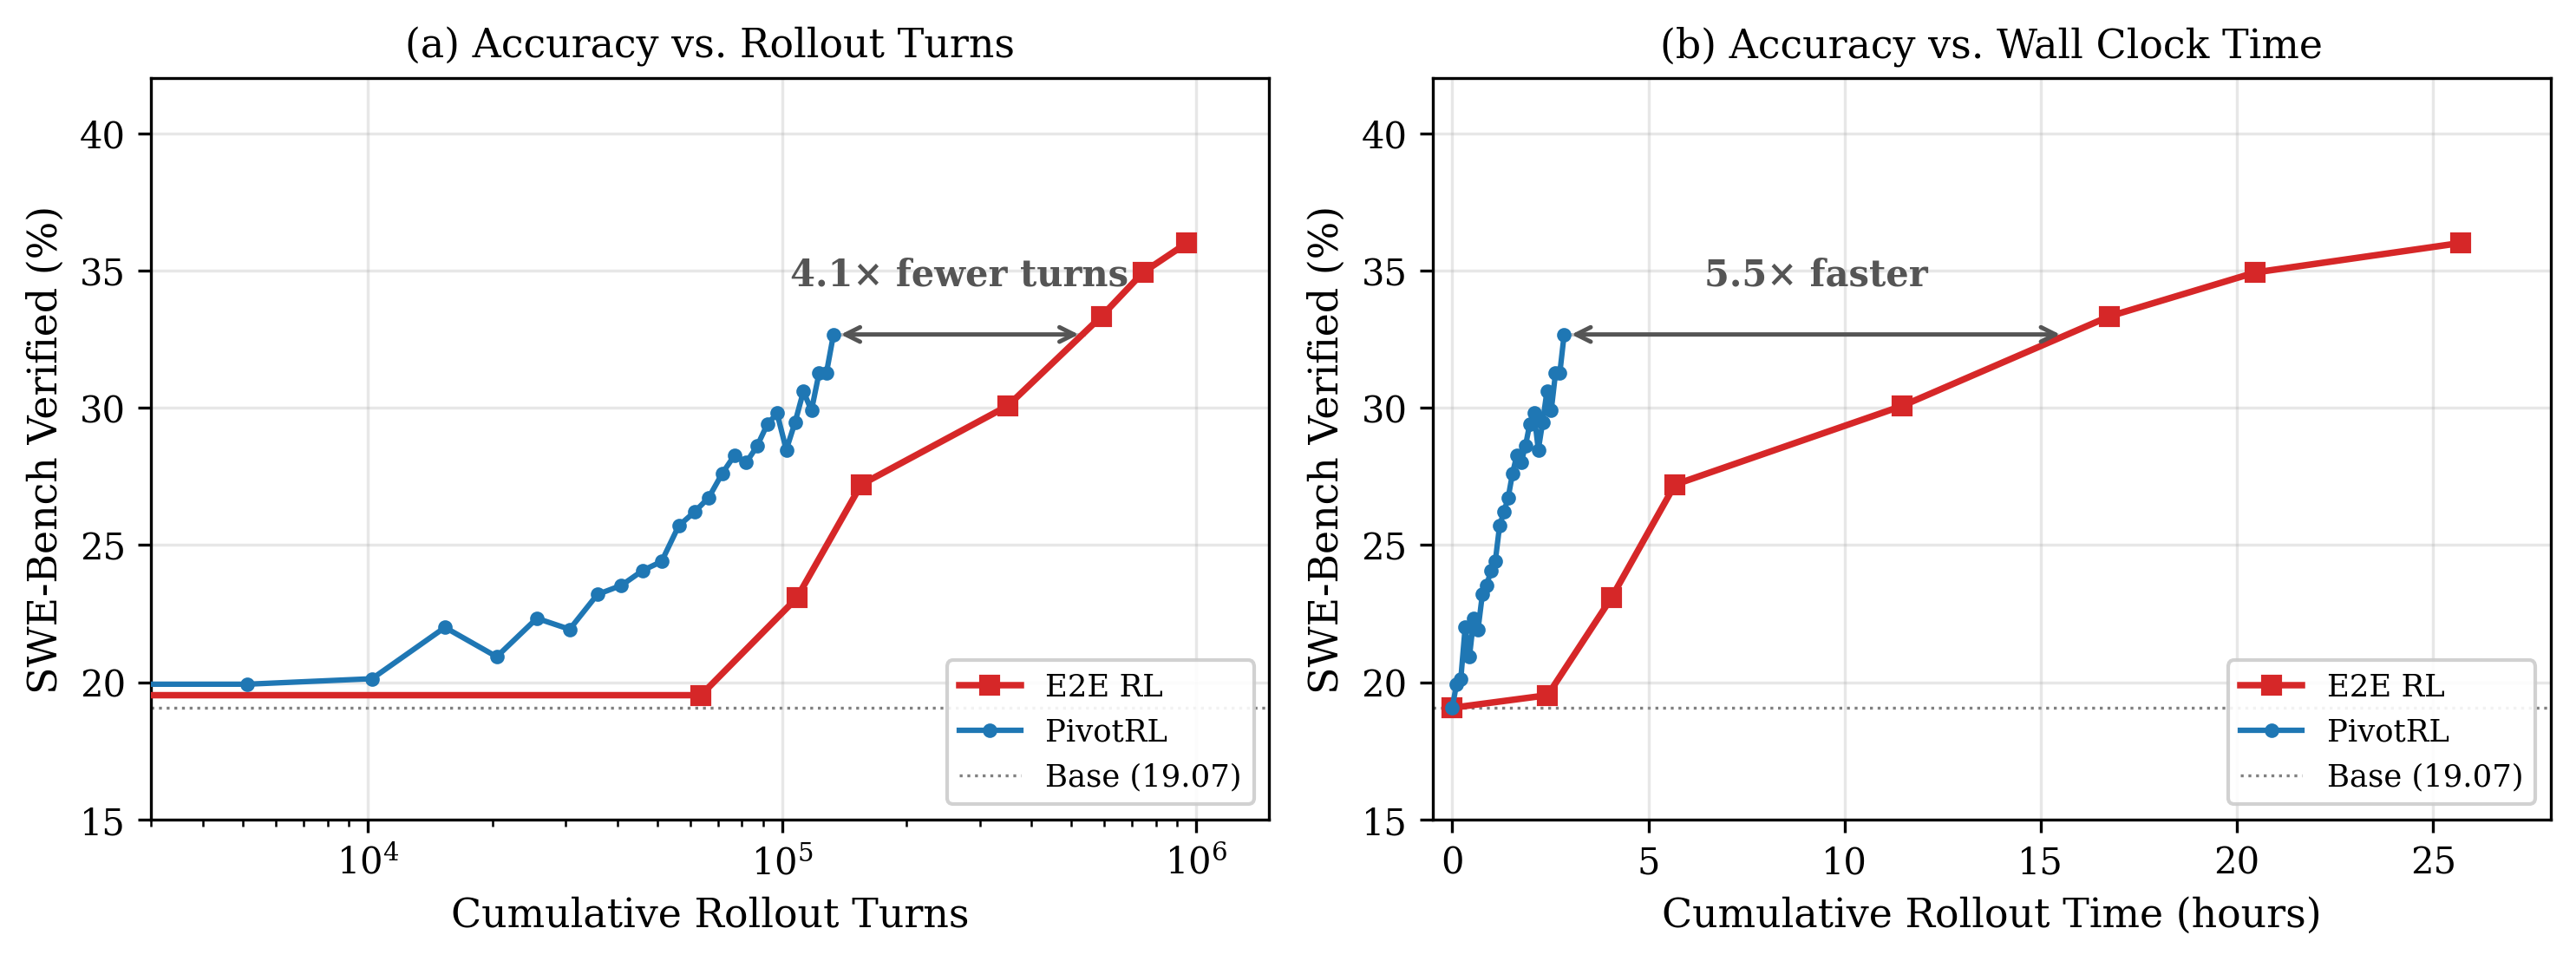
\includegraphics[width=\textwidth]{figures/swe_speedup_v2.png}
    \caption{SWE-Bench 上训练准确率与（a）累计 rollout 轮次数、（b）累计 rollout 时间的关系，所有方法使用相同数量的计算节点。PivotRL 以约 ${\sim}4\times$ 更少的 rollout 轮次数和约 ${\sim}5.5\times$ 更短的训练时间，达到了与 E2E RL 可比的准确率。}
    \label{fig:swe_speedup}
\end{figure*}

\subsection{消融实验}
\label{sec:ablation_study}

我们在表~\ref{tab:ablation_main} 中给出了消融结果。为了分别考察 PivotRL 各个组成部分的贡献，我们在 $\tau^2$-Bench 上每次去掉一个组件。
\begin{table}[t]
\centering
\small
\begin{tabular}{lc}
\toprule
\textbf{配置} & \textbf{$\tau^2$-Bench} \\
\midrule
完整 PivotRL（$\mathcal{D}_{\mathrm{adv}}$ + functional reward） & 63.81 \\
\quad $-$ Pivot 筛选（$\mathcal{D}_{\mathrm{cand}}$ + functional reward） & 59.68 \\
\quad $-$ Functional reward（$\mathcal{D}_{\mathrm{cand}}$ + strict reward） & 57.34 \\
\midrule
同数据 SFT & 58.44 \\
Base & 44.35 \\
\bottomrule
\end{tabular}
\caption{
$\tau^2$-Bench 上的消融结果。Pivot 筛选和功能奖励两者都不可或缺；去掉任意一个都会降低准确率。
}
\label{tab:ablation_main}
\end{table}
去掉筛选后，准确率从 $63.81$ 降到 $59.68$；去掉功能奖励后，结果进一步降到 $57.34$。Pivot 的作用在于把 rollout 集中到那些仍然具有非零优势信号的状态上（命题~\ref{prop:mixed}），而功能奖励则保证了那些虽然文本不同、但语义正确的动作仍然能够获得信用。

图~\ref{fig:tau_pivot_selection_acc} 与图~\ref{fig:tau_reward_std} 展示了这些收益背后的训练动态。在随机采样下，每个 batch 的奖励方差很快塌缩，说明多数被采样到的 pivot 已不再提供有效的优势信号。相比之下，经过筛选的 pivot 集合能够在训练更深阶段维持更高的奖励方差，并优化到更高的验证准确率。

\begin{figure}[t]
    \centering
    \begin{minipage}{0.48\textwidth}
        \centering
        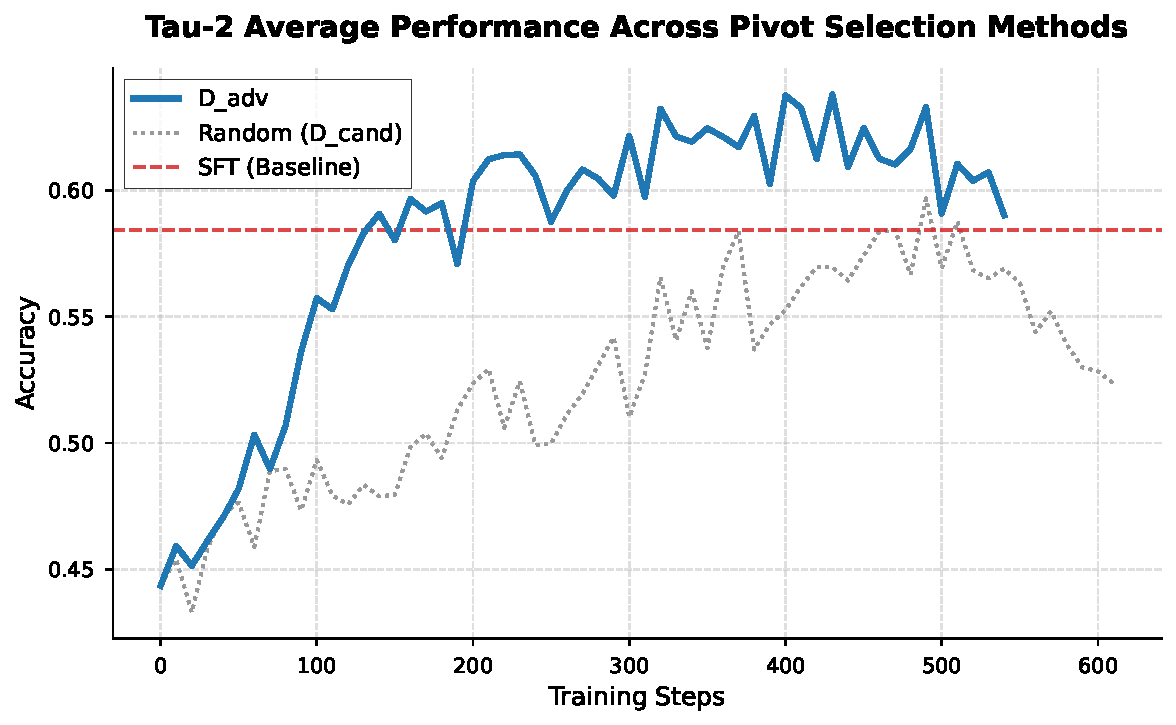
\includegraphics[width=\linewidth]{figures/main_average_validation.pdf}
        \caption{$\tau^2$-Bench 上 RL 训练过程中的准确率。$\mathcal{D}_{adv}$ 的优化效果最强，并优于同数据 SFT。}
        \label{fig:tau_pivot_selection_acc}
    \end{minipage}
    \hfill
    \begin{minipage}{0.48\textwidth}
        \centering
        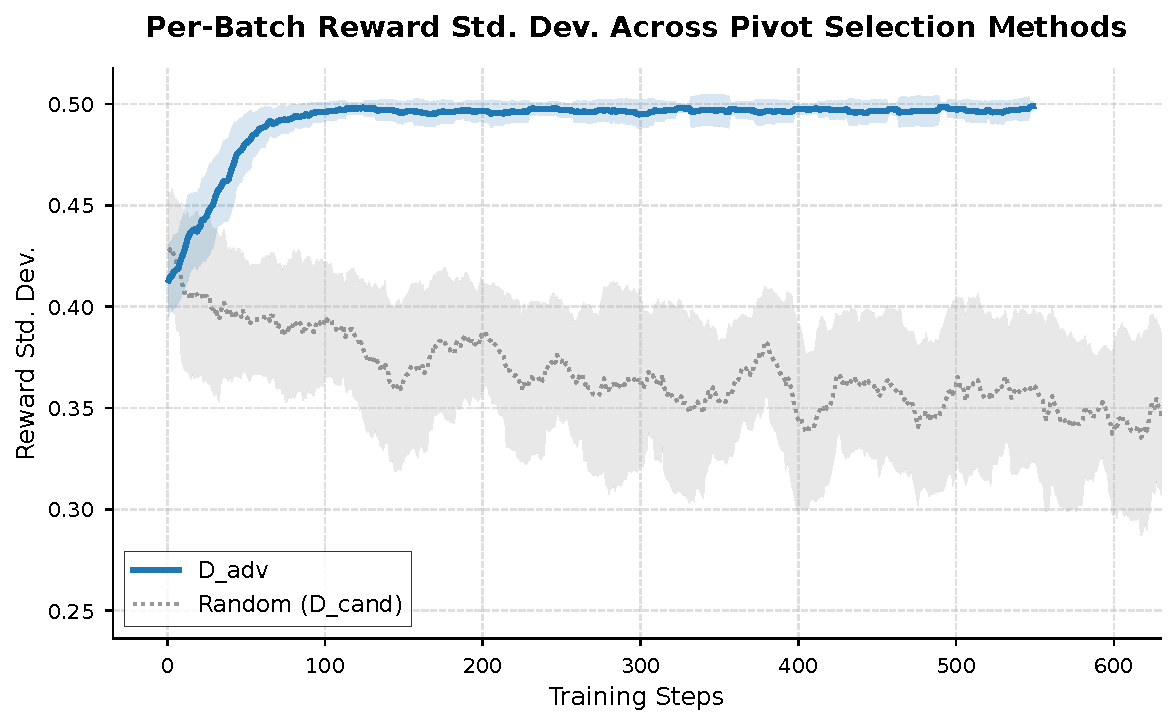
\includegraphics[width=\linewidth]{figures/tau_reward_stddev.pdf}
        \caption{$\tau^2$-Bench 上 RL 训练过程中的奖励标准差。$\mathcal{D}_{adv}$ 维持了更高的奖励方差，因此局部更新信息量也更高。}
        \label{fig:tau_reward_std}
    \end{minipage}
\end{figure}

\subsection{集成到大规模后训练中}
\label{sec:large_scale}

PivotRL 被用于 Nemotron-3-Super 的大规模后训练过程中 \citep{nvidia2025nemotron3super}。表~\ref{tab:large_scale_pivot} 给出了 Nemotron-3-Super 后训练流水线中的智能体基准准确率，其中 PivotRL 负责智能体环境，而其他 RL 环境负责推理与对话。

\begin{table}[t]
\centering
\small
\begin{tabular}{lcc}
\toprule
\textbf{基准} & \textbf{Nemotron-3-Super SFT} & \textbf{经过 PivotRL 阶段后} \\
\midrule
$\tau^2$-Bench         & 48.00 & 64.00 \\
SWE-Bench Verified     & 12.87 & 61.33 \\
Terminal-Bench 1.1 Core & 23.33 & 34.17 \\
BrowseComp             & 13.03 & 25.04 \\
\bottomrule
\end{tabular}
\caption{
Nemotron-3-Super 在 RL 阶段前后的智能体基准准确率。该 RL 阶段在智能体垂直领域中包含 PivotRL 环境，在推理与对话领域中包含其他 RL 环境。
}
\label{tab:large_scale_pivot}
\end{table}
